\documentclass[a4paper,10pt,titlepage]{article}

\usepackage[utf8]{inputenc}
\usepackage{listings}
\usepackage{newclude}
\usepackage{graphicx}
\usepackage{subfigure}
\usepackage{color}

\definecolor{dkgreen}{rgb}{0,0.6,0}
\definecolor{gray}{rgb}{0.5,0.5,0.5}
\definecolor{mauve}{rgb}{0.58,0,0.82}

\lstset{				% must add \usepackage{listings}
  language=C,			% the language of the code
  basicstyle=\footnotesize,	% the size of the fonts that are used for the code
  numbers=left,			% where to put the line-numbers
  numberstyle=\tiny\color{gray},	% the style that is used for the line-numbers
  stepnumber=1,			% the step between two line-numbers. If it's 1, each line will be numbered
  numbersep=5pt,			% how far the line-numbers are from the code
  backgroundcolor=\color{white},% choose the background color. You must add \usepackage{color}
  showspaces=false,		% show spaces adding particular underscores
  showstringspaces=false,		% underline spaces within strings
  showtabs=false,			% show tabs within strings adding particular underscores
  frame=l,				% adds a frame around the code
  rulecolor=\color{black},		% if not set, the frame-color may be changed on line-breaks within not-black text (e.g. commens (green here))
  tabsize=4,				% sets default tabsize to 2 spaces
  captionpos=b,			% sets the caption-position to bottom
  breaklines=true,			% sets automatic line breaking
  breakatwhitespace=false,	% sets if automatic breaks should only happen at whitespace
  title=\lstname,			% show the filename of files included with \lstinputlisting; also try caption instead of title
  keywordstyle=\color{blue},	% keyword style
  commentstyle=\color{dkgreen},% comment style
  stringstyle=\color{mauve},	% string literal style
  escapeinside={\%*}{*)},	% if you want to add a comment within your code
  morekeywords={*,...}		% if you want to add more keywords to the set
}

\title{}


\title{TDT4258 Assignment 2 - Group 1}
\author{Sondre Lefsaker 
  \and André Philipp 
  \and Håvard Wormdal Høiby}

\begin{document}
\maketitle
<<<<<<< HEAD
\newpage
=======
>>>>>>> 257f8d2fc5822703827a298defe206672d69cefb
\section{Abstract}

\tableofcontents
\section{Introduction}
The second assignment introduces us to a new hardware device, the ABDAC. We also utilize
the buttons and LEDs used in assignment one. This gives an introduction to programming with
audio devices and how to produce audio digitally.\\
\\
To the development environment from assignment one we add the GCC C-compiler.\\
\\
The gist of this assignment is to produce different sounds when the buttons on the board are pressed.
The program should be implemented in the C programming language without the support of an
Operation System. We implemented two modes. The first mode is a 7-note piano. The second is a
playback function which plays a different predefined sample for each button. The button SW0
is used to toggle between the two modes.\\
\\
In order to make the program energy efficient the CPU is set to sleep and the DAC is shut 
down while nothing is playing. %a tone is not playing.

\section{Overview}

\section{Solution}
The following sections will describe the different parts of how we implemented the
different parts of the assignment.
\subsection{Button interrupts}
The \textbf{interrupt.c} file has two public functions that is called when an interrupt occurs;
the \textbf{button\_isr} function is called whenever a button is pressed, and
the \textbf{abdac\_isr} function is called regularely at the frequency of the assigned clock.\\
\\
The following code enables interrupts when the buttons is pressed, the first parameter to
the \textbf{register\_interrupt} is the interrupt routine. \\
\begin{lstlisting}
void init_buttons(void) {
	register_interrupt((__int_handler)(button_isr),
			   AVR32_PIOB_IRQ / 32, AVR32_PIOB_IRQ % 32, BUTTONS_INT_LEVEL);
	piob->per = 0xff;
	piob->ier = 0xff;
	piob->puer = 0xff;
}
\end{lstlisting}
The button\_isr function reads from the \textit{isr} register in order to find out what button
is pressed. If SW0 is pressed it switches mode, as described in the previous section,
otherwise it calls a handler function based on if the mode is PIANO\_MODE or PLAYBACK\_MODE.
\begin{lstlisting}
__int_handler *button_isr(void) {
	debounce();

	uint8_t button_interrupt = piob->isr;
	uint8_t button_down = ~(uint8_t)piob->pdsr;
	playing = button_down;

	if ( button_interrupt == SW0 ) {
		if (button_down)
			handle_mode_switch();
	} else {
		if (mode == PIANO_MODE)
			handle_piano_pressed(button_down, button_interrupt);
		else
			handle_sample_pressed(button_down, button_interrupt);
	}

	return 0;
}
\end{lstlisting}
The two handler function \textbf{handle\_piano\_pressed} and \textbf{handle\_sample\_pressed}
pretty much do the same thing; find out what button is pressed and
wake up the abdac if it is sleeping. The handle\_sample\_pressed also resets the currently
playing track (if any) and loads a new track based on the button that was pressed.

\subsection{Sound generation}
To generate sound we used the internal ABDAC (Audio Bitstream Digital-to-Audio-Converter)
on the AVR32 board. It takes a sequence of samples and converts it into an analog
signal, amplifies and outputs it.
The ABDAC uses 2 of the pins on the PIO port B to send signals to the output, and the
6th clock of the Power Manager to generate interrupts that processes the samples.
The clock is set up with oscillator 0 as the source and no division of the frequency.
This gives us a clock of 20 MHz and a sample rate of 20MHz / 256 = 81.920 kHz on the ABDAC\\
Details about these settings was found in the documentation\cite{avr32-stk1000}.
\begin{lstlisting}
	// Register interrupt handler
	register_interrupt((__int_handler)(abdac_isr),
			   AVR32_ABDAC_IRQ / 32, AVR32_ABDAC_IRQ % 32, ABDAC_INT_LEVEL);

	// Disable PIO
	piob->PDR.p20 = 1;
	piob->PDR.p21 = 1;

	// Enable ABDAC
	piob->ASR.p20 = 1;
	piob->ASR.p21 = 1;

	// Set the clock to use Oscillator (OSC0 and OSC1 is 20MHz and 12MHz)
	volatile avr32_pm_t *sm = &AVR32_PM;
	volatile avr32_pm_gcctrl_t *clock = &sm->gcctrl[6];

	clock->oscsel = 0;
	clock->pllsel = 0;
	clock->cen = ON;
\end{lstlisting}
The ABDAC is turned of when it is not used, to save power and keep the output silent.\\
\begin{lstlisting}
	dac->CR.en = OFF;
	dac->IER.tx_ready = OFF;
\end{lstlisting}
To send samples to the ABDAC, in the interrupt routine, each of the stereo-channels are written with the corresponding sample data. We have only used mono sounds in our implementation, so the channels are written with equal samples.\\
\begin{lstlisting}
	dac->SDR.channel0 = sound;
	dac->SDR.channel1 = sound;
\end{lstlisting}
\subsubsection{Piano mode}
The waveforms that are used as base for the samples are sine, triangle, sawtooth, square and white noise. They are implemented in \textbf{samples.c} as mathematical functions of a counter that ticks for a constant length. To make it possible to play multiple tones at once all tones are accumulated to the sample before written to the channels.\\
\begin{lstlisting}
for (i=0; i<7; i++) {
	sound += get_tone_pitch(i);
}
\end{lstlisting}
The get\_tone\_pitch() function loops through all piano key buttons and adds the corresponding tone for the buttons that are pressed.\\
\begin{lstlisting}
static int16_t get_tone_pitch(int i) {
	int16_t sound = 0;
	if ( isDown(i) ) {
		sound = square_sample(samples[i]);
		samples[i] += scale[i];
		if (samples[i] >= SAMPLES) {
			samples[i] = 0;
		}
	}
	return sound;
}
\end{lstlisting}

\subsubsection{Playback mode}
For playing multiple sounds at once in the playback mode, all the tracks are looped and accumulated in the sample.\\
\begin{lstlisting}
for (i=0; i<TRACKS; i++) {
	sound += get_track_pitch(i);
	if (tracks[i] != NULL) {
		notNULL = 1;
	}
}
\end{lstlisting}
The get\_track\_pitch function plays a note for a given duration, the progress is stored in the progress variable. The notes are linked together in a linked list, when the progress of a note is complete (eq. equals the duration) the next note in the list is loaded. When the end of the list is reached (eq. next = NULL) the whole track is done. To prevent the notes from sounding like one long note, the cutoff adds a little pause between each one.
\begin{lstlisting}
static int16_t get_track_pitch(int i) {
	static int samples[TRACKS] = {0, 0, 0, 0};

	int16_t sound = 0;

	// If note is done
	if (tracks[i] && tracks[i]->progress >= tracks[i]->duration) {
		tracks[i]->progress = 0;
		tracks[i] = tracks[i]->next; // Is NULL when tune is done
	}

	// Check if tune is done
	if (tracks[i] == NULL) {

	} else {

		if (tracks[i]->progress <= (int16_t)(tracks[i]->duration * tracks[i]->cutoff) ) {
			sound = (*sample_fn)(samples[i]);
		}

		tracks[i]->progress++;
		samples[i] += tracks[i]->pitch;

		if (samples[i] >= SAMPLES) {
			samples[i] = 0;
		}
	}

	return sound;
}
\end{lstlisting}
\subsection{Setting the frequency}
The \textbf{abdac\_isr} function is, as discussed, called with a frequency of 81.910 kHz. This gives us the sample frequency $ f_s $. To
get a tone frequency, $f_t$ of 440Hz which is the tone A\footnote{440 Hz is called Concert pitch, (``A'' one common tongue) the tone used to tune an ensamble of instruments.},
we have to produce a wave form with this frequency from $f_s$. We generated a sine table with $SAMPLES = 4096$, meaning we
generate 4096 values with even distance from $sin(0)$ to $sin(2\pi)$.\\
\\
If we play the 4096 samples one by one in a loop the $f_t = f_s / SAMPLES = 20Hz$. To set a $f_t$ of choice the following formula
is used:
$$f_t = f_s / (SAMPLES / pitch\_modificator) $$
Calculating this for $f_t = 440 Hz$ gives $pitch\_modificatior \approx 22$. \\
This value was computed after the implementation was done. The implemented valus differs from this slightly\footnote{A is 27} as
it was chosen by trial and error. As correct pitch was not critical the code has not been updated.


\subsection{Making songs and tracks}
A song is created in a similar way to ordinary music.
Given the structure of a music sheet, consisting of several notes with associated
properties and different tracks like bass and main melody,
we are then able to play the same song when it is written in our format. \\
\\
All the songs and predefined music tracks is defined in the \textbf{sounds.c} file.
The following sections sections describes how to create the
Starman Theme Song\cite{smb-starman-theme} from Super Mario Brothers, but the process is the same
for every song.\\
\\
The song has two associated functions; \textbf{init\_smb\_starman\_theme} used to initialize
the song, calculating the different tacks and each note in the song,
and \textbf{smb\_starman\_theme} used by the interrupt-routine to set the playing track
to Starman Theme.\\
\\
\subsubsection{Initializing the song}
The Starman Theme consists of three tracks, two tracks as the main theme and one bass track.
Each track has a associated pointer, this allowes us the calculate each track only
\textit{one} time.
\begin{lstlisting}
	static struct note_t *smb_starman_theme_startT0;
\end{lstlisting}
A track is created with the helper function \textbf{variable\_tune} in the \textbf{notes.c} file.
It is passed a number of parameters, the most important one being an array containing pairs
of \textit{tones} and \textit{durations} defined in \textbf{tones.h}. This is a part of the array
representing the bass in the song:
\begin{lstlisting}
	int pitch_low[114] = {
		PAUSE, EIGHT,
		D2, EIGHT, PAUSE, EIGHT, A2, EIGHT, PAUSE, SIXTEENTH, D3, SIXTEENTH,
		PAUSE, FORTH, A2, EIGHT, D3, EIGHT,
		// ...
	};
\end{lstlisting}
The \textbf{variable\_tune} function is then called with the pitch-array, an integer representing
the number of notes in the song and value for the \textit{cutoff}, respectively. It returns a pointer to the linked list of notes, which is assigned to the respective track pointer in
\textbf{sounds.c}.
\begin{lstlisting}
	smb_starman_theme_startT2 = variable_tune(pitch_low, 57, 0.875);
\end{lstlisting}
\subsubsection{Playing the song}
When the interrupt routine wants to play the track, the \textbf{smb\_starman\_theme} function
is called. All it does is set the type of sample wave for the ABDAC and set the
different tracks in the playback module.
\begin{lstlisting}
	void smb_starman_theme ( void ) {
		set_sample_fn ( square_sample );

		set_track ( 0, smb_starman_theme_startT0 );
		set_track ( 1, smb_starman_theme_startT1 );
		set_track ( 2, smb_starman_theme_startT2 );
	}
\end{lstlisting}
\begin{figure}[h]
	\centerline{{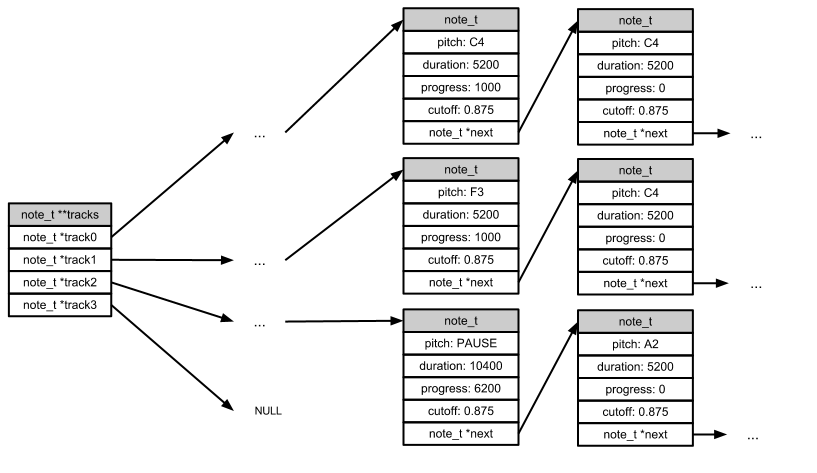
\includegraphics[width=480px]{tracks_example02.png}}}
	\caption{Example of what the tracks array in \textbf{playback.c} may look like}
	\label{tracks-example}
\end{figure}
During execution of the song, the \textbf{tracks} array in \textbf{playback.c}
will look something like Figure[\ref{tracks-example}].
Whenever the progress of a note\_t struct exceeds the duration of the note,
the \textbf{get\_track\_pitch} function will handle the switch
to the next note in the respective track. While one
track switches a note, the other tracks may stay on the same. \\
\\
When all the tracks have reached the end of the linked list we tried to implement a
stop action to turn of the ABDAC (as is done between notes in the piano). This implementation
did not work. But we recognize this is a vital part of a energy efficient system.
 %button - sondre, audio -andy + explotion
\include*{extra}%andy
\section{Test Report}
\begin{table}[h]
  %\centering
  \begin{tabular}{|p{1.1cm}|p{1.5cm}|p{2cm}|p{2cm}|p{2cm}|p{2cm}|}
    \hline
    Number&
    TestCase&
    Prerequisites&
    Input&
    Expected&
    Result\\
    \hline
    1& Startup completed&
    make upload the program, press reset&
    &
    leds 7 and 3 should be on&
    \textcolor{dkgreen}{Passed} 13.03.2012\\
    \hline
    2&
    Piano default mode&
    Startup completed&
    Button SW7 pressed&
    LED7 on and tone playing while button is down&
    \textcolor{dkgreen}{Passed} 13.03.2012\\
    \hline
    3&
    Release piano note&
    SW7 down, piano mode&
    Button SW7 released&
    LED7 off and tone stops playing&
    \textcolor{dkgreen}{Passed} 13.03.2012\\
    \hline
    4&
    Functional piano&
    Startup completed&
    Press button SW7-SW1&
    Dur-scale played&
    \textcolor{dkgreen}{Passed} 13.03.2012\\
    \hline
    5&
    Polytone piano&
    Startup completed&
    Press button SW7 and SW5&
    Base tone and major 3th playing&
    \textcolor{dkgreen}{Passed} 13.03.2012\\

    \hline
    6&
    Switch modes&
    Startup completed&
    Press button SW0&
    All LEDS on&
    \textcolor{dkgreen}{Passed} 13.03.2012\\
    \hline
    7&
    Switch modes back&
    Switch modes&
    Press button SW0&
    All LEDS off, piano active&
    \textcolor{dkgreen}{Passed} 13.03.2012\\
    \hline
    8&
    Play sample&
    Switch modes&
    Press button SW7&
    Sample 7 starts playing&
    \textcolor{dkgreen}{Passed} 13.03.2012\\
    \hline
    9&
    Play another sample&
    While Playing a sample (sample 7)&
    Press button SW6&
    Sample 7 stops playing, sample 6 starts&
    \textcolor{dkgreen}{Passed} 13.03.2012\\
    \hline
    10&
    Switching modes stops sample&
    Playbackmode on, sample is playing&
    Press button SW0&
    Sample stops, mode is piano&
    \textcolor{dkgreen}{Passed} 13.03.2012\\
    \hline

  \end{tabular}
  \caption{Test Report}
\end{table}
%testplan - sondre
\include*{discussion}%andy
\include*{conclusion}%andy
\include*{references}
\end{document}
